% Author: Dominik Harmim <harmim6@gmail.com>


\documentclass[a4paper, 11pt]{article}


\usepackage[utf8]{inputenc}
\usepackage[british]{babel}
\usepackage[left=2cm, top=3cm, text={17cm, 24cm}]{geometry}
\usepackage{times}
\usepackage{graphicx}
\usepackage{amsmath}
\usepackage{enumerate}


\begin{document}


	%%%%%%%%%%%%%%%%%%%%%%%%%%%%%%%% Title page %%%%%%%%%%%%%%%%%%%%%%%%%%%%%%%%
	\begin{titlepage}
		\begin{center}
			
\includegraphics[width=0.5\linewidth]{inc/Bangor_logo.pdf} \\

			\vspace{\stretch{0.382}}

			\LARGE{ICP-2011 -- Computer Networks} \\
			\Huge{\textbf{Assignment -- Review Questions}}

			\vspace{\stretch{0.618}}
		\end{center}

		{\Large
			\today
			\hfill
			Dominik Harmim (eeub8c)
		}
	\end{titlepage}



	%%%%%%%%%%%%%%%%%%%%%%%%%%%%%%%% Answers %%%%%%%%%%%%%%%%%%%%%%%%%%%%%%%%
	\section*{Answers}

	\begin{enumerate}
		\item % 1.
			\textbf{Pure Time Division Multiplexing (TDM)} -- The time slots are allocated on a constant basis.
			This means that user 1 always gets time slot 1, user 2 always gets time slot 2, and so no.
			Provided bandwidth is not used efficiently. There is guaranteed transmission path.

			\textbf{Statistical Time Division Multiplexing (STDM)} -- Allocates bandwidth to each user on the basis
			of demands and needs. A user uses time slots only when they are actually transmitting data.
			When a user is not sending data, no time slots are allocated to it, and other users that
			are sending data can use these time slots. Time slots are allocated statistically.

			$ \text{raw data rate of the user} = B \cdot \frac{1}{T} \, \text{[b]} $ \\
			$ \text{raw data rate of the entire TDM channel} = B \cdot N \cdot \frac{1}{T} \, \text{[b]} $

			$ \text{user A transmission bandwidth} = 10 \cdot 2 = 20 \, \text{[Mb/s]} $ \\
			$ \text{user C transmission bandwidth} = \frac{10}{2} = 5 \, \text{[Mb/s]} $

		\item % 2.
			TODO: Image with matrix is somehow damaged because column parity digits are not visible.

			Parity checking-based error correction technique fails when even number of errors occur.

		\item % 3.
			Data network architecture diagram:
			\begin{figure}[ht]
				\centering
				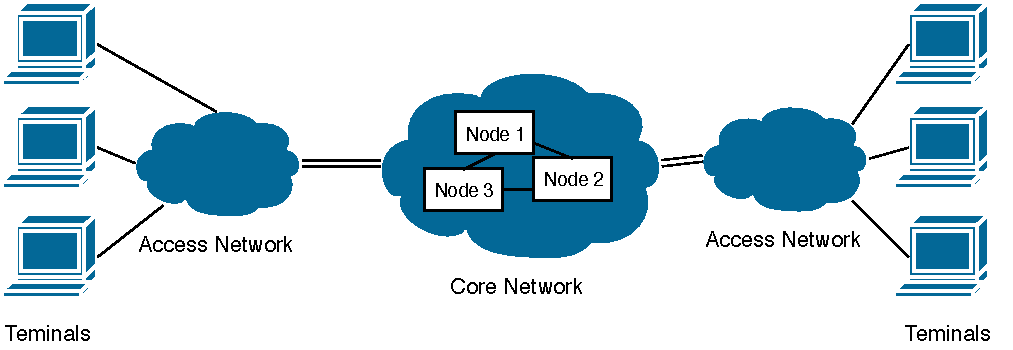
\includegraphics[width=0.7\linewidth]{inc/data_network_architecture.pdf}
				\caption{Data Network Architecture}
				\label{figure:data_network_architecture}
			\end{figure}

			\textbf{Communication protocol} -- Set of rules and procedures describing exchange the information
			within networks. Protocols enables devices to communicate by using set of rules.

			\textbf{Communication architecture} -- Describes special functions that the computer hardware and software
			must perform to allow application programs to communicate with the outside world.
			Communication architecture is based on communication protocol.

		\item % 4.
			OSI reference model layers:
			\begin{enumerate}[1]
				\item % 1.
					Physical Layer
					\begin{description}
						\item vi) Mechanical, electrical and functional interface.
					\end{description}

				\item % 2.
					Data Link Layer
					\begin{description}
						\item i) Error correction and re-transmission.
						\item iv) Responsibility for carrying frames between adjacent nodes.
						\item vii) Flow control.
						\item viv) Three packet switching technologies including X.25, Frame Relay and ATM.
					\end{description}

				\item % 3.
					Network Layer
					\begin{description}
						\item iii) Route determination.
						\item viv) Three packet switching technologies including X.25, Frame Relay and ATM.
					\end{description}

				\item % 4.
					Transport Layer
					\begin{description}
						\item i) Error correction and re-transmission.
						\item vii) Flow control.
						\item viii) Reliable process-to-process message delivery.
					\end{description}

				\item % 5.
					Session Layer
					\begin{description}
						\item ii) Establishing and monitoring an entire communication connection between users.
					\end{description}

				\item % 6.
					Presentation Layer

				\item % 7.
					Application Layer
					\begin{description}
						\item v) Communicates directly with user’s application program.
					\end{description}
			\end{enumerate}

		\item % 5.
			Diagram shows content of packets when computer A sends data to computer D:
			\begin{figure}[ht]
				\centering
				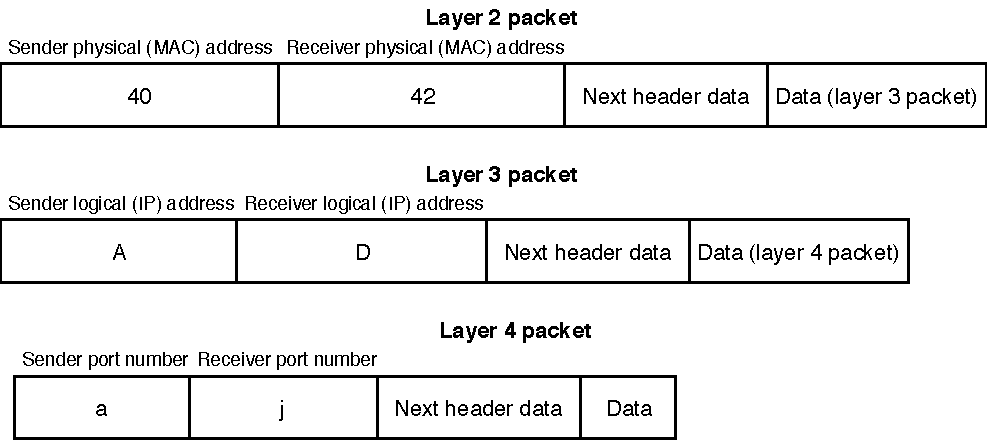
\includegraphics[width=0.7\linewidth]{inc/layer_packets_a_to_d.pdf}
				\caption{Computer A sends data to computer D}
				\label{figure:layer_packets_a_to_d}
			\end{figure}

			Diagram shows content of packets when computer D sends data to computer A:
			\begin{figure}[ht]
				\centering
				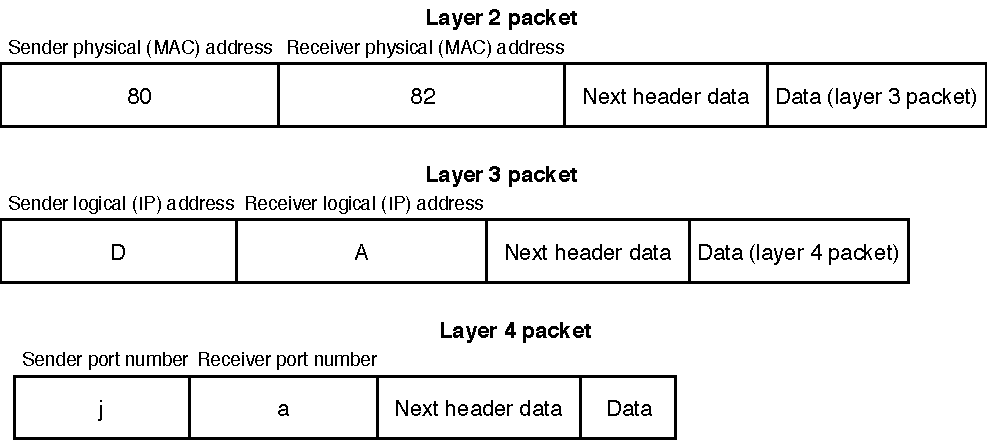
\includegraphics[width=0.7\linewidth]{inc/layer_packets_d_to_a.pdf}
				\caption{Computer D sends data to computer A}
				\label{figure:layer_packets_d_to_a}
			\end{figure}

			Data which sends computer A are encapsulated to layer 4 packet which in addition contains port
			numbers and other header information. Whole layer 4 packet is then encapsulated to layer 3 packet
			which in addition contains logical (IP) addresses and other header information. Finally is whole
			layer 3 packet encapsulated to layer 2 packet which in addition contains physical (MAC) addresses
			and other header information. This layer 2 packet is forwarded to layer 1.

			If the physical destination address of a frame is corrupted during the transmission, the frame will
			be dropped and computer A can be informed about that either when receives this information from device
			that has received this corruption or computer A could waiting for some acknowledgment information which
			has not received.

			Error control mechanisms are still required at layer 4 because sending data are basically divided on multiple
			packets and some of these packets may be dropped, lost or it could be lost their original order and such errors
			could be detected only at layer 4 of receiving side.

		\item % 6.
			TCP in conjunction with IP can ensure the proper message delivery to the destination because TCP operates at
			layer 4 and ensures the reliability of user's message delivery, re-transmit data lost by the lower layers and
			IP operates at layer 3 and is responsible for routing and delivering individual packets.

			Diagram shows relationship between a TCP segment and an IP datagram:
			\begin{figure}[ht]
				\centering
				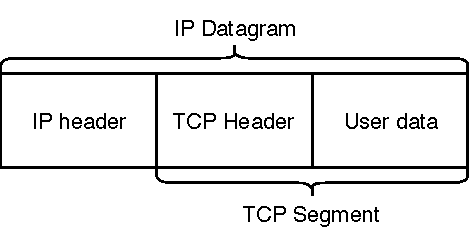
\includegraphics[width=0.4\linewidth]{inc/tcp_ip_relation.pdf}
				\caption{Relationship between a TCP segment and an IP datagram}
				\label{figure:tcp_ip_relation}
			\end{figure}

		\item % 7.
			Diagram of ATM switches:
			\begin{figure}[ht]
				\centering
				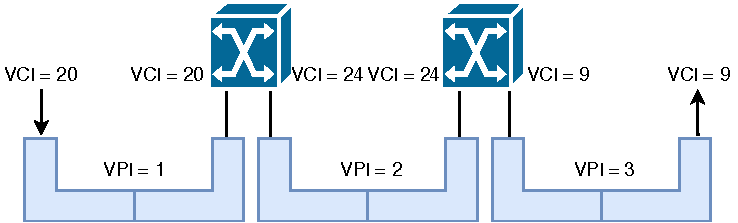
\includegraphics[width=0.7\linewidth]{inc/atm_switch.pdf}
				\caption{ATM switches using both VCI and VPI numbers}
				\label{figure:atm_switch}
			\end{figure}

		\item % 8.
			\textbf{TCP and UDP main differences} -- TCP allows better error checking, more functionality and stability.
			UDP, however, lacks extensive error checking but is considered to be much faster than TCP.
			TCP, unlike UDP, establishes a virtual connection before transmission, guarantees the delivery of data over
			networks and if data is not received correctly, the sending computer will be notified and re-sends the
			information. TCP is connection oriented protocol and UDP is connection-less protocol.

		\item % 9.
			\textbf{Packet switching} -- Information is divided into a number of specially formatted packets, each of
			which includes some addresses such as logical, physical and port addresses. These packets are routed by a
			series of intermediate nodes of the network to the destination. At the destination, received packets are
			reassembled to form the original stream of data.

			\textbf{Connection oriented packet switching} -- End-to-end virtual connection to the destination is
			established using single request packet that contains the source and destination addresses. The subsequent
			packets of the same message just need to carry the marking information, which defines the already established
			virtual connection. There is no need to look at addressing information to calculate a path for each packet,
			the intermediate nodes only read the marking information to route the packet to its destination.

			\textbf{Connection-less packet switching} -- Each packet of a message is an independent unit that contains the
			source and destination addresses. Each packet is independently routed at each intermediate nodes it crosses.

		\item % 10.
			Routing table in a connection-less packet switched network \textbf{can not} have two entries with the same destination
			address because this routing table must unambiguously maps destination addresses to output ports.

			Switching table in a connection oriented packet switched network
			\begin{enumerate}[i)]
				\item \textbf{can} have two entries with the same input VPI,
				\item \textbf{can} have two entries with the same incoming VCI and
				\item \textbf{can not} have two entries with the same incoming VPI and VCI pair.
			\end{enumerate}
	\end{enumerate}


\end{document}
